
%% %%
%% %% INTRO
%% %%

\slide{ A vs C side asymmetry: W vs Z }
{

\only<1>{
 \iteb
 \item 2011 data, MC11c, STACO muons
 \item The plots below show A-side to C-side ratios for data, background-subtracted data, and signal MC.
 \item Standard selection for inclusive W analysis: $p_T^{\mu}>20$, $E_T^{Miss}>25$, $m_T^{W}>40$, iso $p_{T}^{R=40}/p_{T}<0.1$
 \item Single-muon trigger (18 GeV) used both for Ws and Zs
 \item Reconstruction, trigger, isolation scale factors are computed in bins of measurement.
 \item The shaded error bands (on the W plots) include all detector systematics.
 \item We expect that A/C ratio agrees between data and MC within the error bands.
 \item  But... (focus on last 4 \eta\ bins)
 \itee
}
\only<6>{
  \iteb
  \item The overall ``funny'' A/C structure seen in Ws is caused by the trigger and confirmed in Zs.
  \item In Zs, this structure is reasonably well-modeled by the Monte-Carlo.
  \item In Ws, there are multi-sigma A/C disagreements (e.g., last 4 bins in $W^{+}$)
  \item Source of disagreements is not clear: see backup slides for detailed cross-checks.
  \itee
}

\colb[T]

\column{.5\textwidth}
\centering
\only<2>{ \small{ $W^{+}$}}
\only<3>{ \small{ Z, trigger match, 2nd muon anywhere ($\mu^{+}$)}}
\only<4>{ \small{ Z, trigger match, same \eta\ bin ($\mu^{+}$)}}
\only<5>{ \small{ Z, no trigger match ($\mu^{+}$)}}
\includegraphics[width=1.0\textwidth]<2>{dates/20130214/figures/AC/W_NOM_Q4_stack_d3_eta_lpt_met_y_2__1_z_0__1_POS}
\includegraphics[width=1.0\textwidth]<3>{dates/20130214/figures/AC/ZNT_TMATCHBOTH_stack_leptonP_etav_ALL}
\includegraphics[width=1.0\textwidth]<4>{dates/20130214/figures/AC/ZNT_SAME_TMATCHBOTH_stack_leptonP_etav_ALL}
\includegraphics[width=1.0\textwidth]<5>{dates/20130214/figures/AC/ZNT_NOM_stack_leptonP_etav_ALL}

\column{.5\textwidth}
\centering
\only<2>{ \small{ $W^{-}$}}
\only<3>{ \small{ Z, trigger match, 2nd muon anywhere ($\mu^{-}$)}}
\only<4>{ \small{ Z, trigger match, same \eta\ bin ($\mu^{-}$)}}
\only<5>{ \small{ Z, no trigger match ($\mu^{-}$)}}
\includegraphics[width=1.0\textwidth]<2>{dates/20130214/figures/AC/W_NOM_Q4_stack_d3_eta_lpt_met_y_2__1_z_0__1_NEG}
\includegraphics[width=1.0\textwidth]<3>{dates/20130214/figures/AC/ZNT_TMATCHBOTH_stack_leptonN_etav_ALL}
\includegraphics[width=1.0\textwidth]<4>{dates/20130214/figures/AC/ZNT_SAME_TMATCHBOTH_stack_leptonN_etav_ALL}
\includegraphics[width=1.0\textwidth]<5>{dates/20130214/figures/AC/ZNT_NOM_stack_leptonN_etav_ALL}

\cole
}

%%%%%%% Back-up slides %%%%%%%%%%
\appendix
\newcounter{finalframe}
\setcounter{finalframe}{\value{framenumber}}

\slide{}
{

\centering
\Huge Back-up slides
}



%%
%% A/C side differences
%%
\slide{A-C side differences}
{
\centering
\Huge A-C side differences

}

\slide{ Final numbers: A/C for $W^-$ }
{
\small{
\begin{table}[tbph]
\centering
\begin{tabular}{lccccc}
\hline
\hline
$\eta$ bin & $XSEC_{|\eta|}^{ele}$ & $XSEC_{|\eta|}^{\mu}$ & $\delta$ & $XSEC_{Aside} - XSEC_{Cside}$ & $(A-C)/\delta$ \\
\hline

$0 < |\eta| <0.21$ & 433.0 & 431.5 & 4.0 & -9.4 & -2.3 \\
$0.21 < |\eta| <0.42$ & 428.9 & 430.3 & 4.1 & -2.1 & -0.5 \\
$0.42 < |\eta| <0.63$ & 423.8 & 424.6 & 4.7 & -6.8 & -1.5 \\
$0.63 < |\eta| <0.84$ & 418.8 & 418.7 & 3.7 & 6.8 & 1.8 \\
$0.84 < |\eta| <1.05$ & 412.0 & 407.8 & 5.1 & 11.5 & 2.3 \\
$1.05 < |\eta| <1.37$ & 406.2 & 398.8 & 5.1 & 1.4 & 0.3 \\
$1.37 < |\eta| <1.52$ & XXX.X & 380.9 & 4.5 & 1.3 & 0.3 \\
$1.52 < |\eta| <1.74$ & XXX.X & 371.9 & 4.1 & 4.9 & 1.2 \\
$1.74 < |\eta| <1.95$ & 360.4 & 358.0 & 5.1 & 4.3 & 0.9 \\
$1.95 < |\eta| <2.18$ & 339.9 & 331.5 & 3.9 & 19.4 & \color{red}{5.0} \\
$2.18 < |\eta| <2.4$ & XXX.X & 316.4 & 3.6 & -0.5 & -0.1 \\

\hline
\end{tabular}
\caption{Studying A-side vs C-side differences for $W^{-} \rightarrow \mu^{-} \nu$.}
\label{tab:NEG}
\end{table}
}
}

\slide{ Final numbers: A/C for $W^+$ }
{
\small{
\begin{table}[tbph]
\centering
\begin{tabular}{lccccc}
\hline
\hline
$\eta$ bin & $XSEC_{|\eta|}^{ele}$ & $XSEC_{|\eta|}^{\mu}$ & $\delta$ & $XSEC_{Aside} - XSEC_{Cside}$ & $(A-C)/\delta$ \\
\hline

$0 < |\eta| <0.21$ & 572.5 & 570.5 & 4.6 & 1.9 & 0.4 \\
$0.21 < |\eta| <0.42$ & 571.4 & 573.9 & 4.6 & -1.7 & -0.4 \\
$0.42 < |\eta| <0.63$ & 572.5 & 572.9 & 6.9 & 0.8 & 0.1 \\
$0.63 < |\eta| <0.84$ & 579.0 & 578.0 & 4.5 & 14.3 & \color{red}{3.2} \\
$0.84 < |\eta| <1.05$ & 582.6 & 577.9 & 5.2 & 7.1 & 1.4 \\
$1.05 < |\eta| <1.37$ & 596.2 & 589.2 & 5.7 & 8.9 & 1.6 \\
$1.37 < |\eta| <1.52$ & XXX.X & 586.2 & 6.2 & 7.3 & 1.2 \\
$1.52 < |\eta| <1.74$ & XXX.X & 586.9 & 5.4 & 26.5 & \color{red}{4.9} \\
$1.74 < |\eta| <1.95$ & 596.9 & 591.2 & 4.2 & 13.3 & \color{red}{3.1} \\
$1.95 < |\eta| <2.18$ & 584.8 & 570.7 & 7.0 & 32.4 & \color{red}{4.6} \\
$2.18 < |\eta| <2.4$ & XXX.X & 558.3 & 6.4 & 10.2 & 1.6 \\

\hline
\end{tabular}
\caption{Studying A-side vs C-side differences for $W^{+} \rightarrow \mu^{+} \nu$.}
\label{tab:POS}
\end{table}
}
}

\slide{ A-C ratios: data-driven vs MC QCD }
{

\only<1>{
 A/C ratios for data, background-subtracted data, and signal MC. \\
 The shaded errors on the ratio (in the following plots) are correct. \\
 Here, we are considering the \red{effects of QCD subtraction}. \\
 \small{(the fits, however, are always performed in an integrated kinematic region)}
}
\only<5>{
  Conclusion: on the scale of existing A/C disagreements, the choice of QCD templates is a minor effect. \\
  All subsequent plots will use simple, unscaled QCD-based template (bb/cc mu15X) to study A/C differences.
}

\colb[T]

\column{.5\textwidth}
\centering
\only<2>{ \small{ Data-driven QCD (global fit): $W^{+}$}}
\only<3>{ \small{ Data-driven QCD (per-bin fit): $W^{+}$}}
\only<4>{ \small{ Heavy-flavor MC QCD: $W^{+}$}}
\includegraphics[width=1.0\textwidth]<2>{dates/20130214/figures/AC/W_NOM_Q4_stack_d3_eta_lpt_met_y_2__1_z_0__1_POS}
\includegraphics[width=1.0\textwidth]<3>{dates/20130214/figures/AC/W_NOM_Q4BINS_stack_d3_eta_lpt_met_y_2__1_z_0__1_POS}
\includegraphics[width=1.0\textwidth]<4>{dates/20130214/figures/AC/W_NOM_Q0_stack_d3_eta_lpt_met_y_2__1_z_0__1_POS}

\column{.5\textwidth}
\centering
\only<2>{ \small{ Data-driven QCD (global fit): $W^{-}$}}
\only<3>{ \small{ Data-driven QCD (per-bin fit): $W^{-}$}}
\only<4>{ \small{ Heavy-flavor MC QCD: $W^{-}$}}
\includegraphics[width=1.0\textwidth]<2>{dates/20130214/figures/AC/W_NOM_Q4_stack_d3_eta_lpt_met_y_2__1_z_0__1_NEG}
\includegraphics[width=1.0\textwidth]<3>{dates/20130214/figures/AC/W_NOM_Q4BINS_stack_d3_eta_lpt_met_y_2__1_z_0__1_NEG}
\includegraphics[width=1.0\textwidth]<4>{dates/20130214/figures/AC/W_NOM_Q0_stack_d3_eta_lpt_met_y_2__1_z_0__1_NEG}

\cole
}


\slide{ A-C ratios: choice of signal MC }
{

\only<1>{
 A/C ratios for data, background-subtracted data, and signal MC. \\
 The shaded errors on the ratio (in the following plots) are correct. \\
 Here, we are considering the \red{effects of different signal MCs}. \\
 \small{(for all subsequent studies, MC-based QCD will be used for simplicity)}
}
\only<5>{
  Conclusion: A/C disagreements persist for all generators.
}

\colb[T]

\column{.5\textwidth}
\centering
\only<2>{ \small{ Nominal: $W^{+}$}}
\only<3>{ \small{ Powheg-Herwig: $W^{+}$}}
\only<4>{ \small{ MCNLO: $W^{+}$}}
\includegraphics[width=1.0\textwidth]<2>{dates/20130214/figures/AC/W_NOM_Q0_stack_d3_eta_lpt_met_y_2__1_z_0__1_POS}
\includegraphics[width=1.0\textwidth]<3>{dates/20130214/figures/AC/WSYS_BGSIG4_Q0_stack_d3_eta_lpt_met_y_2__1_z_0__1_POS}
\includegraphics[width=1.0\textwidth]<4>{dates/20130214/figures/AC/WSYS_BGSIG1_Q0_stack_d3_eta_lpt_met_y_2__1_z_0__1_POS}

\column{.5\textwidth}
\centering
\only<2>{ \small{ Nominal: $W^{-}$}}
\only<3>{ \small{ Powheg-Herwig: $W^{-}$}}
\only<4>{ \small{ MCNLO: $W^{-}$}}
\includegraphics[width=1.0\textwidth]<2>{dates/20130214/figures/AC/W_NOM_Q0_stack_d3_eta_lpt_met_y_2__1_z_0__1_NEG}
\includegraphics[width=1.0\textwidth]<3>{dates/20130214/figures/AC/WSYS_BGSIG4_Q0_stack_d3_eta_lpt_met_y_2__1_z_0__1_NEG}
\includegraphics[width=1.0\textwidth]<4>{dates/20130214/figures/AC/WSYS_BGSIG1_Q0_stack_d3_eta_lpt_met_y_2__1_z_0__1_NEG}

\cole
}


\slide{ A-C ratios: playing with reco/trigger scale factors }
{

\only<1>{
 A/C ratios for data, background-subtracted data, and signal MC. \\
 The shaded errors on the ratio (in the following plots) are correct. \\
 Here, we are considering the \red{effects of reco/trigger scale factors}. \\
 \small{(sorry, no systematic bands in the following set of plots)}
}
\only<6>{
  Conclusion: trigger scale factors have a major effect, especially in the barrel. \\
  However, they don't seen to provide a substantial A/C correction in the endcaps. \\
  (i.e., forward TGC trigger chambers are more symmetric than RPCs in the barrel)
}


\colb[T]

\column{.5\textwidth}
\centering
\only<2>{ \small{ Nominal: $W^{+}$}}
\only<3>{ \small{ Without reco SF: $W^{+}$}}
\only<4>{ \small{ Without trigger SF: $W^{+}$}}
\only<5>{ \small{ Without either SF: $W^{+}$}}
\includegraphics[width=1.0\textwidth]<2>{dates/20130214/figures/AC/WNT_NOM_Q0_stack_lepton_etav_POS}
\includegraphics[width=1.0\textwidth]<3>{dates/20130214/figures/AC/WNT_NORECSF_Q0_stack_lepton_etav_POS}
\includegraphics[width=1.0\textwidth]<4>{dates/20130214/figures/AC/WNT_NOTRIGSF_Q0_stack_lepton_etav_POS}
\includegraphics[width=1.0\textwidth]<5>{dates/20130214/figures/AC/WNT_NOSF_Q0_stack_lepton_etav_POS}

\column{.5\textwidth}
\centering
\only<2>{ \small{ Nominal: $W^{-}$}}
\only<3>{ \small{ Without reco SF: $W^{-}$}}
\only<4>{ \small{ Without trigger SF: $W^{-}$}}
\only<5>{ \small{ Without either SF: $W^{-}$}}
\includegraphics[width=1.0\textwidth]<2>{dates/20130214/figures/AC/WNT_NOM_Q0_stack_lepton_etav_NEG}
\includegraphics[width=1.0\textwidth]<3>{dates/20130214/figures/AC/WNT_NORECSF_Q0_stack_lepton_etav_NEG}
\includegraphics[width=1.0\textwidth]<4>{dates/20130214/figures/AC/WNT_NOTRIGSF_Q0_stack_lepton_etav_NEG}
\includegraphics[width=1.0\textwidth]<5>{dates/20130214/figures/AC/WNT_NOSF_Q0_stack_lepton_etav_NEG}

\cole
}


\slide{ A-C ratios: playing with kinematic regions }
{

\only<1>{
 A/C ratios for data, background-subtracted data, and signal MC. \\
 The shaded errors on the ratio (in the following plots) are correct. \\
 Here, we are considering the \red{effects of different kinematic cuts}. \\
 \small{(sorry, no systematic bands in the following set of plots)}
}
\only<5>{
  Conclusion: disagreements persist even in higher-pT kinematic regions.
}

\colb[T]

\column{.5\textwidth}
\centering
\only<2>{ \small{ Nominal: $p_T>20, met>25, wmt>40$, $W^{+}$}}
\only<3>{ \small{ Nominal: $p_T>25, met>25, wmt>40$, $W^{+}$}}
\only<4>{ \small{ Nominal: $p_T>20, met>35, wmt>50$, $W^{+}$}}
\includegraphics[width=1.0\textwidth]<2>{dates/20130214/figures/AC/WNT_NOM_Q0_stack_lepton_etav_POS}
\includegraphics[width=1.0\textwidth]<3>{dates/20130214/figures/AC/WNT_PT25_Q0_stack_lepton_etav_POS}
\includegraphics[width=1.0\textwidth]<4>{dates/20130214/figures/AC/WNT_MET35WMT50_Q0_stack_lepton_etav_POS}

\column{.5\textwidth}
\centering
\only<2>{ \small{ Nominal: $p_T>20, met>25, wmt>40$, $W^{-}$}}
\only<3>{ \small{ Nominal: $p_T>25, met>25, wmt>40$, $W^{-}$}}
\only<4>{ \small{ Nominal: $p_T>20, met>35, wmt>50$, $W^{-}$}}
\includegraphics[width=1.0\textwidth]<2>{dates/20130214/figures/AC/WNT_NOM_Q0_stack_lepton_etav_NEG}
\includegraphics[width=1.0\textwidth]<3>{dates/20130214/figures/AC/WNT_PT25_Q0_stack_lepton_etav_NEG}
\includegraphics[width=1.0\textwidth]<4>{dates/20130214/figures/AC/WNT_MET35WMT50_Q0_stack_lepton_etav_NEG}

\cole
}


\slide{ A-C ratios: trigger matching in W }
{

\only<1>{
 A/C ratios for data, background-subtracted data, and signal MC. \\
 The shaded errors on the ratio (in the following plots) are correct. \\
 Here, we are considering the \red{effect of requiring the W muon trigger match}. \\
 \small{(sorry, no systematic bands in the following set of plots)}
}

\only<4>{
  Conclusion: as expected, requiring the W muon to explicitly match a trigger \red{does not do anyting} - because in an over-whelming majority of cases, that W muon had to fire the trigger anyway.
}

\colb[T]

\column{.5\textwidth}
\centering
\only<2>{ \small{ Nominal, $W^{+}$}}
\only<3>{ \small{ Nominal + trigger match, $W^{+}$}}
\includegraphics[width=1.0\textwidth]<2>{dates/20130214/figures/AC/WNT_NOM_Q0_stack_lepton_etav_POS}
\includegraphics[width=1.0\textwidth]<3>{dates/20130214/figures/AC/WNT_TRIGMATCH_Q0_stack_lepton_etav_POS}

\column{.5\textwidth}
\centering
\only<2>{ \small{ Nominal, $W^{-}$}}
\only<3>{ \small{ Nominal + trigger match, $W^{-}$}}
\includegraphics[width=1.0\textwidth]<2>{dates/20130214/figures/AC/WNT_NOM_Q0_stack_lepton_etav_NEG}
\includegraphics[width=1.0\textwidth]<3>{dates/20130214/figures/AC/WNT_TRIGMATCH_Q0_stack_lepton_etav_NEG}

\cole
}


\slide{ A-C ratios: choice of MET }
{

\only<1>{
 A/C ratios for data, background-subtracted data, and signal MC. \\
 The shaded errors on the ratio (in the following plots) are correct. \\
 Here, we are considering the \red{effects of a different MET definitions}. \\
 \small{Option 1: MetRefFinal, but without correcting for muon/jet momentum } \\
 \small{Option 2: LocHadTopo (corrected for muons), as used in the 2010 measurement} \\
 \small{(sorry, no systematic bands in the following set of plots)}
}

\only<5>{
  Conclusion: disagreements persist even with other METs. \\
  However, things move around a bit ($W^+$ gets better, $W^-$ gets worse), which is caused not by the choice of MET but by whether the muon momentum scale corrections are propagated into MET. As will be shown later, this is the effect of the charge-splitting curvature correction.
}

\colb[T]

\column{.5\textwidth}
\centering
\only<2>{ \small{ Nominal: MetRefFinal, $W^{+}$}}
\only<3>{ \small{ Nominal: MetRefFinal (uncorr), $W^{+}$}}
\only<4>{ \small{ Nominal: LocHadTopo+mu (uncorr), $W^{+}$}}
\includegraphics[width=1.0\textwidth]<2>{dates/20130214/figures/AC/WNT_NOM_Q0_stack_lepton_etav_POS}
\includegraphics[width=1.0\textwidth]<3>{dates/20130214/figures/AC/WNT_RAWMET_Q0_stack_lepton_etav_POS}
\includegraphics[width=1.0\textwidth]<4>{dates/20130214/figures/AC/WNT_METLH_Q0_stack_lepton_etav_POS}

\column{.5\textwidth}
\centering
\only<2>{ \small{ Nominal: MetRefFinal, $W^{-}$}}
\only<3>{ \small{ Nominal: MetRefFinal (uncorr), $W^{-}$}}
\only<4>{ \small{ Nominal: LocHadTopo+mu (uncorr), $W^{-}$}}
\includegraphics[width=1.0\textwidth]<2>{dates/20130214/figures/AC/WNT_NOM_Q0_stack_lepton_etav_NEG}
\includegraphics[width=1.0\textwidth]<3>{dates/20130214/figures/AC/WNT_RAWMET_Q0_stack_lepton_etav_NEG}
\includegraphics[width=1.0\textwidth]<4>{dates/20130214/figures/AC/WNT_METLH_Q0_stack_lepton_etav_NEG}

\cole
}


\slide{ A-C ratios: $d_0$ cut }
{

\only<1>{
 A/C ratios for data, background-subtracted data, and signal MC. \\
 The shaded errors on the ratio (in the following plots) are correct. \\
 Here, we are considering the \red{effect of adding a $|d_{0}/d_{0}^{sig}|<3.5$ cut}. \\
 \small{ this is the same cut that's used in the Z channel }
}

\only<4>{
  Conclusion: disagreements persist even with a $d_0$-significance cut.
}

\colb[T]

\column{.5\textwidth}
\centering
\only<2>{ \small{ Nominal $W^{+}$}}
\only<3>{ \small{ Nominal + d0, $W^{+}$}}
\includegraphics[width=1.0\textwidth]<2>{dates/20130214/figures/AC/W_NOM_Q4_stack_d3_eta_lpt_met_y_2__1_z_0__1_POS}
\includegraphics[width=1.0\textwidth]<3>{dates/20130214/figures/AC/WSYS_D0_Q0_stack_d3_eta_lpt_met_y_2__1_z_0__1_POS}

\column{.5\textwidth}
\centering
\only<2>{ \small{ Nominal $W^{-}$}}
\only<3>{ \small{ Nominal + d0, $W^{-}$}}
\includegraphics[width=1.0\textwidth]<2>{dates/20130214/figures/AC/W_NOM_Q4_stack_d3_eta_lpt_met_y_2__1_z_0__1_NEG}
\includegraphics[width=1.0\textwidth]<3>{dates/20130214/figures/AC/WSYS_D0_Q0_stack_d3_eta_lpt_met_y_2__1_z_0__1_NEG}

\cole
}


\slide{ A-C ratios: muon momentum corrections }
{

\only<1>{
 A/C ratios for data, background-subtracted data, and signal MC. \\
 The shaded errors on the ratio (in the following plots) are correct. \\
 Here, we are considering the \red{effect of muon momentum corrections}. \\
 \small{Reminder: muon momentum corrections are split into ``K'' (overall $p_T$ scale) and ``C'' (curvature splitting).}
}
\only<10>{
  Conclusion: while muon momentum corrections have an effect on the A/C disagreements, there is no version of correction factors
that exhibits good agreement for both $W^+$ and $W^-$. Various versions simply provide a play-off between better agreement for $mu^+$ versus $mu^-$, which is mainly influenced by the propagation of curvature correction (``C'') into MET.
}

\colb[T]

\column{.5\textwidth}
\centering
\only<2>{ \small{ Nominal $W^{+}$}}
\only<3>{ \small{ Nominal, no C $W^{+}$}}
\only<4>{ \small{ Nominal, no C, no K $W^{+}$}}
\only<5>{ \small{ Nominal (repeated): $W^{+}$}}
\only<6>{ \small{ Corrections in fine eta bins: $W^{+}$}}
\only<7>{ \small{ Nominal (repeated): $W^{+}$}}
\only<8>{ \small{ Corrections from Higgs note (no C): $W^{+}$}}
\only<9>{ \small{ Nominal, no C (repeated) $W^{+}$}}
\includegraphics[width=1.0\textwidth]<2>{dates/20130214/figures/AC/W_NOM_Q4_stack_d3_eta_lpt_met_y_2__1_z_0__1_POS}
\includegraphics[width=1.0\textwidth]<3>{dates/20130214/figures/AC/WSYS_MCPNOC_Q0_stack_d3_eta_lpt_met_y_2__1_z_0__1_POS}
\includegraphics[width=1.0\textwidth]<4>{dates/20130214/figures/AC/WSYS_MCPNOCK_Q0_stack_d3_eta_lpt_met_y_2__1_z_0__1_POS}
\includegraphics[width=1.0\textwidth]<5>{dates/20130214/figures/AC/W_NOM_Q4_stack_d3_eta_lpt_met_y_2__1_z_0__1_POS}
\includegraphics[width=1.0\textwidth]<6>{dates/20130214/figures/AC/WSYS_MCPFINE_Q0_stack_d3_eta_lpt_met_y_2__1_z_0__1_POS}
\includegraphics[width=1.0\textwidth]<7>{dates/20130214/figures/AC/W_NOM_Q4_stack_d3_eta_lpt_met_y_2__1_z_0__1_POS}
\includegraphics[width=1.0\textwidth]<8>{dates/20130214/figures/AC/WSYS_MCPHIGGS_Q0_stack_d3_eta_lpt_met_y_2__1_z_0__1_POS}
\includegraphics[width=1.0\textwidth]<9>{dates/20130214/figures/AC/WSYS_MCPNOC_Q0_stack_d3_eta_lpt_met_y_2__1_z_0__1_POS}

\column{.5\textwidth}
\centering
\only<2>{ \small{ Nominal $W^{-}$}}
\only<3>{ \small{ Nominal, no C $W^{-}$}}
\only<4>{ \small{ Nominal, no C, no K $W^{-}$}}
\only<5>{ \small{ Nominal (repeated): $W^{-}$}}
\only<6>{ \small{ Corrections in fine eta bins: $W^{-}$}}
\only<7>{ \small{ Nominal (repeated): $W^{-}$}}
\only<8>{ \small{ Corrections from Higgs note (no C): $W^{-}$}}
\only<9>{ \small{ Nominal, no C (repeated) $W^{-}$}}
\includegraphics[width=1.0\textwidth]<2>{dates/20130214/figures/AC/W_NOM_Q4_stack_d3_eta_lpt_met_y_2__1_z_0__1_NEG}
\includegraphics[width=1.0\textwidth]<3>{dates/20130214/figures/AC/WSYS_MCPNOC_Q0_stack_d3_eta_lpt_met_y_2__1_z_0__1_NEG}
\includegraphics[width=1.0\textwidth]<4>{dates/20130214/figures/AC/WSYS_MCPNOCK_Q0_stack_d3_eta_lpt_met_y_2__1_z_0__1_NEG}
\includegraphics[width=1.0\textwidth]<5>{dates/20130214/figures/AC/W_NOM_Q4_stack_d3_eta_lpt_met_y_2__1_z_0__1_NEG}
\includegraphics[width=1.0\textwidth]<6>{dates/20130214/figures/AC/WSYS_MCPFINE_Q0_stack_d3_eta_lpt_met_y_2__1_z_0__1_NEG}
\includegraphics[width=1.0\textwidth]<7>{dates/20130214/figures/AC/W_NOM_Q4_stack_d3_eta_lpt_met_y_2__1_z_0__1_NEG}
\includegraphics[width=1.0\textwidth]<8>{dates/20130214/figures/AC/WSYS_MCPHIGGS_Q0_stack_d3_eta_lpt_met_y_2__1_z_0__1_NEG}
\includegraphics[width=1.0\textwidth]<9>{dates/20130214/figures/AC/WSYS_MCPNOC_Q0_stack_d3_eta_lpt_met_y_2__1_z_0__1_NEG}

\cole
}


\slide{ A-C ratios: W vs Z }
{

\only<1>{
 A/C ratios for data, background-subtracted data, and signal MC. \\
 The shaded errors on the ratio (in the following plots) are correct. \\
 Here, we are comparing \red{W and Z eta plots}. \\
 \small{(sorry, no error band for the Z)}
}
\only<8>{
  Conclusion: when the Z muons are required to trigger, we see the same overall A/C structure as in Ws - which means that the \red{A/C structure is caused by the trigger}. However, the MC models these disagreements reasonably well in Z events, but not in W events. \\
  \small{Caveat: I am not using official trigger matching, but rather \red{manually} match muons to EF trigger objects using a $\phi-\eta$ cone of 0.2.} \\
 
}

\colb[T]

\column{.5\textwidth}
\centering
\only<2>{ \small{ $W^{+}$}}
\only<3>{ \small{ Z, no trigger match ($\mu^{+}$)}}
\only<4>{ \small{ Z, no trigger match, same \eta\ bin ($\mu^{+}$)}}
\only<5>{ \small{ Z, trigger match, same \eta\ bin ($\mu^{+}$)}}
\only<6>{ \small{ Z, trigger match, 2nd muon anywhere ($\mu^{+}$)}}
\only<7>{ \small{ $W^{+}$ (repeated)}}
\includegraphics[width=1.0\textwidth]<2>{dates/20130214/figures/AC/W_NOM_Q4_stack_d3_eta_lpt_met_y_2__1_z_0__1_POS}
\includegraphics[width=1.0\textwidth]<3>{dates/20130214/figures/AC/ZNT_NOM_stack_leptonP_etav_ALL}
\includegraphics[width=1.0\textwidth]<4>{dates/20130214/figures/AC/ZNT_SAME_stack_leptonP_etav_ALL}
\includegraphics[width=1.0\textwidth]<5>{dates/20130214/figures/AC/ZNT_SAME_TMATCHBOTH_stack_leptonP_etav_ALL}
\includegraphics[width=1.0\textwidth]<6>{dates/20130214/figures/AC/ZNT_TMATCHBOTH_stack_leptonP_etav_ALL}
\includegraphics[width=1.0\textwidth]<7>{dates/20130214/figures/AC/WNT_NOM_Q0_stack_lepton_etav_POS}

\column{.5\textwidth}
\centering
\only<2>{ \small{ $W^{-}$}}
\only<3>{ \small{ Z, no trigger match ($\mu^{-}$)}}
\only<4>{ \small{ Z, no trigger match, same \eta\ bin ($\mu^{+}$)}}
\only<5>{ \small{ Z, trigger match, same \eta\ bin ($\mu^{+}$)}}
\only<6>{ \small{ Z, trigger match, 2nd muon anywhere ($\mu^{+}$)}}
\only<7>{ \small{ $W^{-}$ (repeated)}}
\includegraphics[width=1.0\textwidth]<2>{dates/20130214/figures/AC/W_NOM_Q4_stack_d3_eta_lpt_met_y_2__1_z_0__1_NEG}
\includegraphics[width=1.0\textwidth]<3>{dates/20130214/figures/AC/ZNT_NOM_stack_leptonN_etav_ALL}
\includegraphics[width=1.0\textwidth]<4>{dates/20130214/figures/AC/ZNT_SAME_stack_leptonN_etav_ALL}
\includegraphics[width=1.0\textwidth]<5>{dates/20130214/figures/AC/ZNT_SAME_TMATCHBOTH_stack_leptonN_etav_ALL}
\includegraphics[width=1.0\textwidth]<6>{dates/20130214/figures/AC/ZNT_TMATCHBOTH_stack_leptonN_etav_ALL}
\includegraphics[width=1.0\textwidth]<7>{dates/20130214/figures/AC/WNT_NOM_Q0_stack_lepton_etav_NEG}

\cole
}


%% W in slices of PHI

\slide{ A-C ratios: W in different $\phi$ quadrants}
{

\only<1>{
 A/C ratios for data, background-subtracted data, and signal MC. \\
 The shaded errors on the ratio (in the following plots) are correct. \\
 Here, we are comparing W eta plots in different \red{$\phi$ quadrants}.\\
 \small{Caveat: all scale factors are integrated in $\phi$, so we don't expect excellent agreement here}
}
\only<7>{
 Conclusion: the A-C ratio shows very different structure in $\phi$. However, the last four $\eta$ bins of $W^{+}$ show \red{consistent disagreement in ALL four $\phi$ quadrants}.
}

\colb[T]

\column{.5\textwidth}
\centering
\only<2>{ \small{ $W^{+}$ (all $\phi$)}}
\only<3>{ \small{ $W^{+}$ ($0 < \phi < PI/2$)}}
\only<4>{ \small{ $W^{+}$ ($PI/2 < \phi < PI$)}}
\only<5>{ \small{ $W^{+}$ ($-PI < \phi < -PI/2$)}}
\only<6>{ \small{ $W^{+}$ ($-PI/2 < \phi < 0$)}}
\includegraphics[width=1.0\textwidth]<2>{dates/20130214/figures/AC/WNT_NOM_Q0_stack_lepton_etav_POS}
\includegraphics[width=1.0\textwidth]<3>{dates/20130214/figures/AC2_NOM/WNT_NOM_C0_stack_lepton_etav_POS}
\includegraphics[width=1.0\textwidth]<4>{dates/20130214/figures/AC2_NOM/WNT_NOM_C1_stack_lepton_etav_POS}
\includegraphics[width=1.0\textwidth]<5>{dates/20130214/figures/AC2_NOM/WNT_NOM_C2_stack_lepton_etav_POS}
\includegraphics[width=1.0\textwidth]<6>{dates/20130214/figures/AC2_NOM/WNT_NOM_C3_stack_lepton_etav_POS}

\column{.5\textwidth}
\centering
\only<2>{ \small{ $W^{-}$ (all $\phi$)}}
\only<3>{ \small{ $W^{-}$ ($0 < \phi < PI/2$)}}
\only<4>{ \small{ $W^{-}$ ($PI/2 < \phi < PI$)}}
\only<5>{ \small{ $W^{-}$ ($-PI < \phi < -PI/2$)}}
\only<6>{ \small{ $W^{-}$ ($-PI/2 < \phi < 0$)}}
\includegraphics[width=1.0\textwidth]<2>{dates/20130214/figures/AC/WNT_NOM_Q0_stack_lepton_etav_NEG}
\includegraphics[width=1.0\textwidth]<3>{dates/20130214/figures/AC2_NOM/WNT_NOM_C0_stack_lepton_etav_NEG}
\includegraphics[width=1.0\textwidth]<4>{dates/20130214/figures/AC2_NOM/WNT_NOM_C1_stack_lepton_etav_NEG}
\includegraphics[width=1.0\textwidth]<5>{dates/20130214/figures/AC2_NOM/WNT_NOM_C2_stack_lepton_etav_NEG}
\includegraphics[width=1.0\textwidth]<6>{dates/20130214/figures/AC2_NOM/WNT_NOM_C3_stack_lepton_etav_NEG}

\cole
}


%% Explicitly looking inside the bad bins

\slide{ Various distributions for $|\eta| = 1.95-2.18$ (worst bin) }
{

\only<1>{
 Here, we are looking at various distributions inside the worst eta slice: $|\eta| = 1.95-2.18$.\\
 \small{Note that the worst data/MC disagreement is seen on the C-side}
}
\only<10>{
 Conclusions: \\
 In MET and $\phi$ distributions \red{on the C side}, we simply see an overall 5\% shift. \\
 In MET-MuonBoy, we also see some shape differences between A and C sides. \\
 We also see a difference in the correction to MET due to propagation of muon momentum into MET (mostly influenced by the curvature ``C''). This difference is about \red{0.1-0.2 GeV}, which is consistent with the A-C side difference seen in curvature correction constants for combined muons. Recall that those constants are derived by balancing the momenta of the Z boson legs against each other for events where both legs fall in the same $\eta$ bin.
}

\colb[T]

\column{.5\textwidth}
\centering
\only<2>{ \small{ $W^{+}$: muon $\phi$ (C-side)}}
\only<3>{ \small{ $W^{+}$: muon $\phi$ (A-side)}}
\only<4>{ \small{ $W^{+}$: MET (C-side)}}
\only<5>{ \small{ $W^{+}$: MET (A-side)}}
\only<6>{ \small{ $W^{+}$: MET-MuonBoy (C-side)}}
\only<7>{ \small{ $W^{+}$: MET-MuonBoy (A-side)}}
\only<8>{ \small{ $W^{+}$: $\Delta(MET)$ MCP corrections (C-side)}}
\only<9>{ \small{ $W^{+}$: $\Delta(MET)$ MCP correctoins (A-side)}}
\includegraphics[width=1.0\textwidth]<2>{dates/20130214/figures/AC2_NOM/WDB_C_BADBIN_stack_l_phi_POS}
\includegraphics[width=1.0\textwidth]<3>{dates/20130214/figures/AC2_NOM/WDB_A_BADBIN_stack_l_phi_POS}
\includegraphics[width=1.0\textwidth]<4>{dates/20130214/figures/AC2_NOM/WDB_C_BADBIN_stack_met_POS}
\includegraphics[width=1.0\textwidth]<5>{dates/20130214/figures/AC2_NOM/WDB_A_BADBIN_stack_met_POS}
\includegraphics[width=1.0\textwidth]<6>{dates/20130214/figures/AC2_NOM/WDB_C_BADBIN_stack_met_muonboy_POS}
\includegraphics[width=1.0\textwidth]<7>{dates/20130214/figures/AC2_NOM/WDB_A_BADBIN_stack_met_muonboy_POS}
\includegraphics[width=1.0\textwidth]<8>{dates/20130214/figures/AC2_NOM/WDB_C_BADBIN_stack_metcorr_total_POS}
\includegraphics[width=1.0\textwidth]<9>{dates/20130214/figures/AC2_NOM/WDB_A_BADBIN_stack_metcorr_total_POS}

\column{.5\textwidth}
\centering
\only<2>{ \small{ $W^{-}$: muon $\phi$ (C-side)}}
\only<3>{ \small{ $W^{-}$: muon $\phi$ (A-side)}}
\only<4>{ \small{ $W^{-}$: MET (C-side)}}
\only<5>{ \small{ $W^{-}$: MET (A-side)}}
\only<6>{ \small{ $W^{-}$: MET-MuonBoy (C-side)}}
\only<7>{ \small{ $W^{-}$: MET-MuonBoy (A-side)}}
\only<8>{ \small{ $W^{-}$: $\Delta(MET)$ MCP corrections (C-side)}}
\only<9>{ \small{ $W^{-}$: $\Delta(MET)$ MCP corrections (A-side)}}
\includegraphics[width=1.0\textwidth]<2>{dates/20130214/figures/AC2_NOM/WDB_C_BADBIN_stack_l_phi_NEG}
\includegraphics[width=1.0\textwidth]<3>{dates/20130214/figures/AC2_NOM/WDB_A_BADBIN_stack_l_phi_NEG}
\includegraphics[width=1.0\textwidth]<4>{dates/20130214/figures/AC2_NOM/WDB_C_BADBIN_stack_met_NEG}
\includegraphics[width=1.0\textwidth]<5>{dates/20130214/figures/AC2_NOM/WDB_A_BADBIN_stack_met_NEG}
\includegraphics[width=1.0\textwidth]<6>{dates/20130214/figures/AC2_NOM/WDB_C_BADBIN_stack_met_muonboy_NEG}
\includegraphics[width=1.0\textwidth]<7>{dates/20130214/figures/AC2_NOM/WDB_A_BADBIN_stack_met_muonboy_NEG}
\includegraphics[width=1.0\textwidth]<8>{dates/20130214/figures/AC2_NOM/WDB_C_BADBIN_stack_metcorr_total_NEG}
\includegraphics[width=1.0\textwidth]<9>{dates/20130214/figures/AC2_NOM/WDB_A_BADBIN_stack_metcorr_total_NEG}

\cole
}

\slide{A-C cross-check in Wenu channel}
{
Unfolded cross-sections in the Wenu channel on A vs C sides, and their ratio. \\
The disagreement is less than 2\%, as contrasted to up to 5\% in Wmunu channel.

\centering
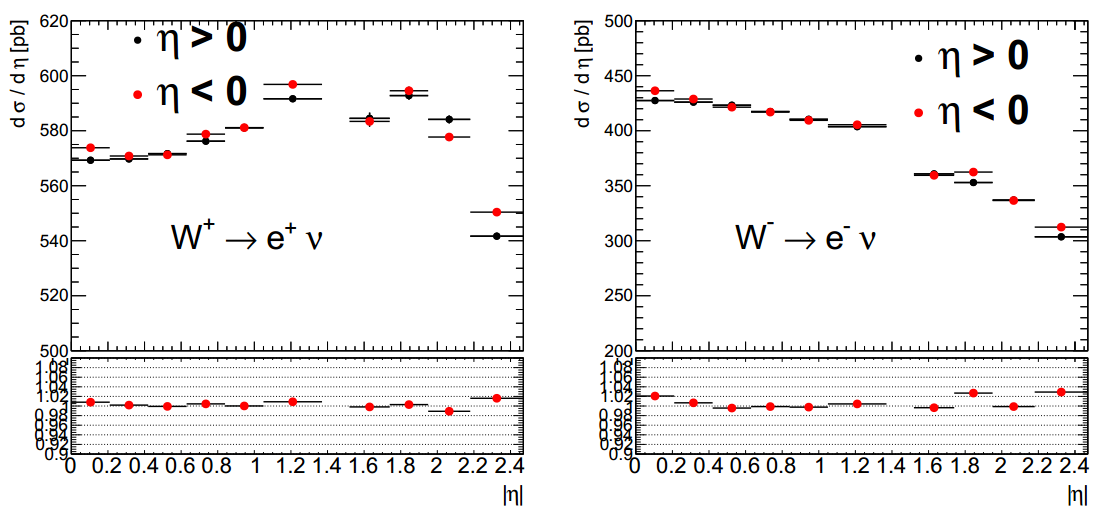
\includegraphics[width=0.8\textwidth]{dates/20130214/figures/ele/Wenu_AC_unfolded}

}


\slide{Conclusions}
{
\centering
It is still unclear what causes the A/C side disagreements in the forward region. \\
Since only Ws are affected, the suspicion falls on MET (MuonBoy term?). \\
But how can we better understand and, ultimately, correct these effects?
}
